
\documentclass{hogent-article}

\usepackage{lipsum} 

\PaperTitle{Onderzoek van de Log4shell kwetsbaarheid met een PoC en de impact die deze aanvallen hebben op de huidige cybersecurity implementaties.}

\PaperType{Paper Research Methods: onderzoeksvoorstel}


\Authors{Kadir Akkurt\textsuperscript{1}, Thomas Thomas\textsuperscript{2}} % Authors


\CoPromotor{}


\affiliation{
    \textsuperscript{1} \href{mailto:kadir.akkurt@student.hogent.be}{kadira.akkurt@student.hogent.be}
}
\affiliation{
    \textsuperscript{2} \href{mailto:thomas.thomas@student.hogent.be}{thomas.thoma@student.hogent.be}
}

\Abstract{

De ernstige Log4shell kwetsbaarheid die vatbaar is voor Remote-Code-Execution (RCE) werd op 10 december 2021 openbaar gemaakt. Er wordt gebruik gemaakt van een bug in de wijdverspreide Log4j-bibliotheek. Elke service die de bibliotheek gebruikt en een interface met internet blootstelt is potentieel kwetsbaar. Er wordt onderzocht wat het Log4j framework en de Log4shell kwetsbaarheid juist is en hoe we deze kwetsbaarheid kunnen uitbuiten, detecteren en bestrijden. In een verder onderzoek gaan we de impact op bedrijfsniveau analyseren. 
Er word verwacht dat de exploit nog steeds veel bedrijven zal treffen en dat bedrijven niet genoeg investeren in cybersecurity.    
}


\Keywords{Cybersecurity; Log4shell; Log4j; Apache; Applicatieontwikkeling; Java; Systeembeheer; Netwerkbeheer}
\newcommand{\keywordname}{Sleutelwoorden} 

\begin{document}

\flushbottom 
\maketitle 
\tableofcontents 
\thispagestyle{empty} 

\section{Inleiding}

Log4J behoort tot een van de zwaarste cyberdreigingen van de laatste decennia en heeft miljoenen computers getroffen. Dit heeft een enorme impact over hoe het cybersecurity landschap evolueert en hoe het zal gevormd worden. Ondanks de gevaren van soortgelijke exploits, investeren bedrijven nog steeds niet genoeg in cybersecurity.
In dit onderzoek word er gekeken wat de impact is van een Log4shell exploit op bedrijven op financieel en technisch vlak, zodat bedrijven aan de hand van de resultaten zelf kunnen beslissen om te investeren in cybersecurity .

\subsection{Log4j framework}

Log4j is een Java-logging-framework dat gedistribueerd wordt onder de Apache Software Licence ~\autocite{Apache2022a}. Het framework is volledig in Java~\autocite{Oracle2022} geschreven en werd origineel ontwikkeld door Ceki Gülcü ~\autocite{Gülcü2002}.

Log4j wordt onder andere gebruikt voor het loggen van foutmeldingen in verschillende softwarepaketten van bekende fabrikanten, waaronder Amazon, Apple iCloud, Cisco, Cloudflare, ElasticSearch, Red Hat, Steam, Tesla, Twitter, en videospelletjes zoals Minecraft. De volledige database is ondergebracht bij ~\textcite{CISA2022} en ~\textcite{NCSCN2022}.

\subsection{Log4j kwetsbaarheid}

De Log4j of LogJam kwetsbaarheid (CVE-2021-44228) ~\autocite{Apache2022c} is een zero-day software kwetsbaarheid in Apache Log4j 2, waarbij cyberaanvallers in staat zijn arbitraire code van op afstand uit te voeren. Deze CVE-2021-44228 kwetsbaarheid die in bepaalde versies ~\autocite{Apache2022b} van Log4j aanwezig is maakt het de aanvaller mogelijk om de controle van een apparaat op het internet over te nemen.  
De kwetsbaarheid bestond onopgemerkt sinds 2013 en werd op 24 november 2021 door Chen Zhaojun van het beveiligingsteam van Alibaba Cloud ontdekt en onthuld aan de Apache Software Foundation, waarvan Log4j een project is.
Op 9 december 2021 publiceerde Apache de publiekelijke bekendmaking van de CVE-2021-44228 die de naam de Log4shell meekreeg samen met een maximale severity score (CVSS \autocite{FIRST2022}) van 10.
In figuur ~\ref{fig:log4shell-tijdlijn} kan je een tijdlijn terugvinden met de belangrijkste vaststellingen rond het Log4shell gebeuren volgens ~\textcite{Hiesgen2022}. 

\begin{figure}[!ht]
    \centering
    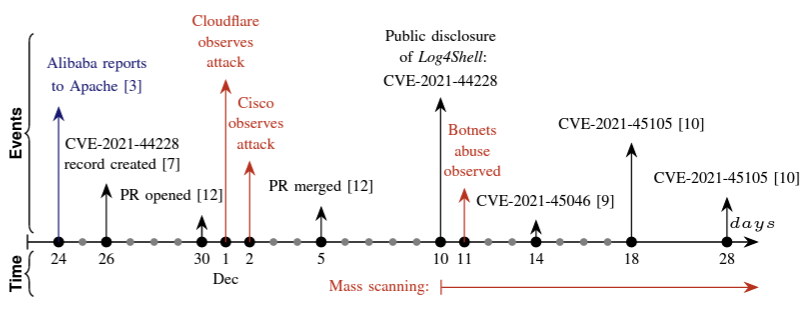
\includegraphics[width=1\linewidth]{img/log4shell-tijdlijn.png}
    \caption{Tijdlijn van de Log4shell ontdekking met de belangrijkste vaststellingen volgens ~\autocite{Hiesgen2022}.}
    \label{fig:log4shell-tijdlijn}
\end{figure} 

Hier stopt het niet en enkele dagen later worden er opnieuw enkele kwetsbaarheden vrijgegeven, nl. CVE-2021-45046 \autocite{Apache2022d}, CVE-2021-4104 \autocite{Apache2022e} en CVE-2021-45105 \autocite{Apache2022f} die respectievelijk per type kwetsbaarheid en getroffen versies in bijhorende Tabel~\ref{tab:CVE-list} verder omschreven is en via de security advisor van The Apache Software Foundation terug te vinden zijn.\autocite{Apache2022b}

\begin{table}[]
    \caption[CVE-list]{Gepubliceerde Log4j CVE's van 10/12/2021 tot 18/12/2021 met type kwetsbaarheid en de getroffen versies.}
    \begin{tabular}{@{}lll@{}}
        \toprule
        \textbf{CVE}   & \textbf{Type Kwetsbaarheid}    & \textbf{Log4j Versies}    \\ \midrule
        CVE-2021-44228 & RCE                            & 2.0 - 2.14.1              \\
        CVE-2021-45046 & DoS en RCE                     & 2.0 - 2.15.0              \\
        CVE-2021-4104  & RCE                            & 1.2 (EOL)                 \\
        CVE-2021-45105 & DoS                            & 2.0-b9 - 2.16.0           \\ \bottomrule
    \end{tabular}
    \label{tab:CVE-list}
    
    {\bf Belangrijke opmerkingen met de Tabel:}
    \begin{itemize}[leftmargin=*]
        \item CVE-2021-44228 is altijd exploiteerbaar wanneer Log4j versies 2.0 t.e.m. 2.14.1 opgenomen zijn.
        \item CVE-2021-45046, CVE-2021-4104 en CVE-2021-45105 kunnen enkel in niet-standaard configuraties voorkomen.
        \item CVE-2021-4104 wordt niet meer gepatcht, omdat de Log4j 1.x-tak End-of-Life (EOL) is.
    \end{itemize}
\end{table}

Voor deze opdracht zijn wij echter vooral geïnteresseerd in de Log4shell kwetsbaarheid (CVE-2021-44228), omdat deze de grootste impact heeft en deze vatbaar is op alle Log4j standaard configuraties met versienummering 2.0 t.e.m. 2.14.1 als een bibliotheek in applicaties of diensten opgenomen is.

\subsection{Log4shell}

Hoewel cyberaanvallers eenvoudig de gegevens van uw organisatie en werknemers kunnen vastleggen via blootgestelde servers, kunnen ze ook schadelijke software installeren op apparaten in uw IT-infrastructuur.

Voor organisaties brengt het gebruik van Log4j-logboek\-registratie in een slecht beveiligde IT-infrastructuur grote risico's met zich mee, met als voorbeeld de diefstal van gevoelige gegevens en de mogelijkheid dat servers en apparaten onbruikbaar worden. Om de schade die Log4j aan organisaties kan toebrengen beter te begrijpen, is het nuttig om uitgebreid te kijken naar het werkingsprincipe van de betreffende bibliotheek en de omgevingen die het beïnvloedt.

Hoewel het ontwikkelaarsteam van Log4j aankondigde dat ze in 2015 stopten met werken voor de eerste versie. Dit op Java gebaseerde logboekbibliotheek wordt vandaag de dag nog steeds veel gebruikt met Log4j-versies 2 en 2.14.1. Het Github-project van Apache Log4j werd door meer dan 400.000 mensen gedownload.

Het moet ook opgemerkt worden dat met de beëindiging van Log4j in 2015 gebruikers werden aangemoedigd om Log4j versie 2 te gebruiken. Met deze stimulans zijn veel instellingen en ontwikkelaars gemigreerd naar Log4j 2 en latere versies. De kwetsbaarheid is ontdekt in versie 2 van Log4j. Dit laat zien dat de systemen die we momenteel gebruiken, van cloud platformen tot webapplicaties, te maken hebben met ernstige beveiligingsproblemen.Technologiebedrijven zoals Amazon, Apple, Twitter, Baidu, Minecraft en Tesla behoren tot de bedrijven die getroffen zijn door de kwetsbaarheid.Daarnaast wordt gesteld dat bedrijven die technologische oplossingen bieden aan bedrijven zoals Oracle, Cisco en IBM ook getroffen kunnen worden door de kwetsbaarheid.

\subsection{Gevaren van Log4shell}

Log4shell is een kwetsbaarheid van het Remote Code Execution (RCE)-type en is een van de gevaarlijkste types van computerkwetsbaarheden. Een aanvaller kan van op afstand kwaadaardige code uitvoeren binnen het doelsysteem op het lokale netwerk of via het Internet. Dit betekent dat er geen fysieke toegang tot het apparaat nodig is om getroffen servers en andere apparaten in de IT-infrastructuur te infecteren met schadelijke software.

Als aanvallers erin slagen deze kwetsbaarheid op een van de servers uit te buiten, krijgen ze de mogelijkheid om willekeurige code uit te voeren en mogelijk de volledige controle van het systeem over te nemen.

Een RCE-kwetsbaarheid kan bijvoorbeeld leiden tot:
    \begin{itemize}[leftmargin=*]
    \item verlies van controle over het systeem of de afzonderlijke componenten ervan;
    \item diefstal van gevoelige gegevens;
    \item systemen uitschakelen door DDOS aanvallen;
    \item softwarematige infiltratie met als doel cryptomining;
    \item aanvallen op supply chains;
    \item uitrollen van malware zoals ransomware.
\end{itemize}

Andere bekende voorbeelden van RCE aanvallen zijn:
\begin{itemize}[leftmargin=*]
    \item CVE-2014-6271 (Shellshock) ~\autocite{Debian2021};
    \item CVE-2017-0147 of MS17-010 (Eternal Blue) ~\autocite{Microsoft2022};
    \item CVE-2022-22965 (Spring4Shell) ~\autocite{VMware2022}.
\end{itemize}

Een ander punt wat de CVE-2021-44228 zo gevaarlijk maakt is de eenvoud van de hack. Zo moeten aanvallers de Log4j applicatie alleen maar dwingen om een string naar het logboek te laten schrijven en daarna kunnen ze al hun kwaadaardige code in de applicatie gaan uploaden via de message lookup substitution-functie.

Beveiligingsbedrijf Check Point omschrijft dit beveiligingslek als een Cyberpandemie en doet registraties van aanvalspogingen die pieken tot meer dan 100 per minuut ~\autocite{Checkpoint2021}.

\begin{figure}[!ht]
    \centering
    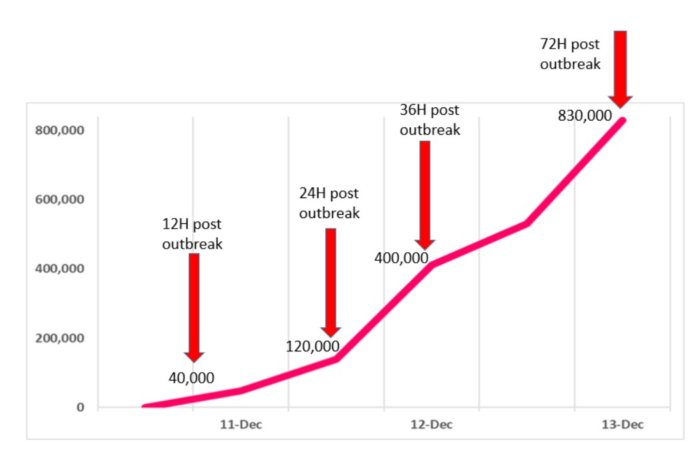
\includegraphics[width=1\linewidth]{img/aanvallen72h.png}
    \caption{Evolutie geregistreerde Log4shell aanvalspogingen door ~\textcite{Checkpoint2021} van 11/12/2021 tot 13/12/2021.}
    \label{fig:aanvallen72h}
\end{figure}
Checkpoint, dat een oplossing biedt voor het probleem van het uitvoeren van code met toegang op afstand, stelt dat er in 72 uur meer dan 830.000 aanvallen hebben plaatsgevonden (Figuur ~\ref{fig:aanvallen72h}). Aanvallers richten zich vooral op bedrijfsnetwerken. Er moet ook worden opgemerkt dat het Apache-team Log4j versie 2.15.0 heeft uitgebracht door een patch te maken om de bovengenoemde kwetsbaarheid te verminderen.

\subsection{Werking Log4shell hack}

\begin{itemize}[leftmargin=*]
    \item JNDI
\end{itemize}

Iedere java client kan JNDI (Java Naming and Directory Interface) ~\autocite{Oracle2020} gebruiken om gegevens bij een Directory Service op te halen door een bepaalde naam de definiëren.
Wanneer een aanvaller deze naam kan wijzigen, zodat er gegevens opgehaald kunnen worden, dan kan hij er ook voor kiezen om deze te verwijzen naar een server naar keuze die dan het gewenste Java object laat terugsturen. Wanneer het Java object gevonden wordt gaat dit geladen worden op het systeem.

\begin{itemize}[leftmargin=*]
    \item LDAP
\end{itemize}

Het LDAP (Lightweight Directory Access Protocol) wordt gebruikt voor het beheer van gebruikers en bepaalde systeembronnen ~\autocite{Microsoft2018}.
LDAP biedt een manier van directory-opslag door de combinatie van authentificatie van gebruikers en autorisatie tot externe bronnen.

\begin{itemize}[leftmargin=*]
    \item JNDI vs LDAP
\end{itemize}

Een aanvaller kan dus JNDI en LDAP laten samenwerken ~/autocite{Oracle2020} om gegevens op te halen uit deze directory services en het is deze Log4j kwetsbaarheid die misbruikt wordt ~\autocite{Conikee2021}.

\begin{itemize}[leftmargin=*]
\item Voorbeeld:
\end{itemize}

In Figuur ~\ref{fig:jndi-ldaplookup} zie je een voorbeeld van de aanval die in de PoC ~\autocite{Akkurt2022} volledig verder uitgewerkt is.

\begin{figure}[!ht]
    \centering
    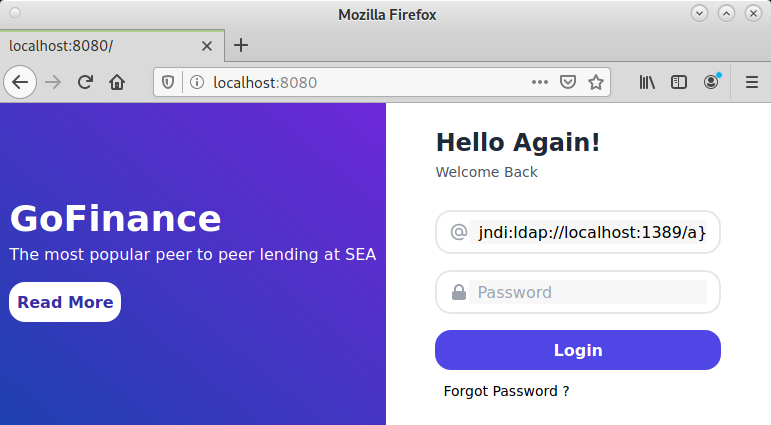
\includegraphics[width=1\linewidth]{img/jndi-ldaplookup.png}
    \caption{Log4shell aanval op een lokaal draaiende webapplicatie die de kwetsbare Log4j versie gebruikt om de gebruikersinvoer te loggen.}
    \label{fig:jndi-ldaplookup}
\end{figure}

\begin{itemize}[leftmargin=*]
    \item Log4j intern
\end{itemize}

Log4j herkent eerst de syntax \verb|\${}| en gaat deze formatteren, vervolgens gaat de ``key'' \verb|jndi| herkent worden en weet Log4j dat er een JndiLookup moet gebeuren.

Hierna wordt er dan een verbinding gemaakt met de LDAP-server van de aanvaller (payload).

De LDAP server gaat een link teruggeven naar een locatie waar de gevraagde bron kan worden gedownload, 
zoals bijvoorbeeld een HTTP server met de kwaadaardige code. 

Log4j gaat de code dan downloaden en uitvoeren zodat de hacker volledige toegang krijgt tot het systeem dat deze applicatie gebruikt.

In Figuur\ref{fig:log4shell-schema} kan je een schematische voorstelling van een Log4shell aanval terugvinden ~\autocite{Zscaler2021}.

\begin{figure}[!ht]
    \centering
    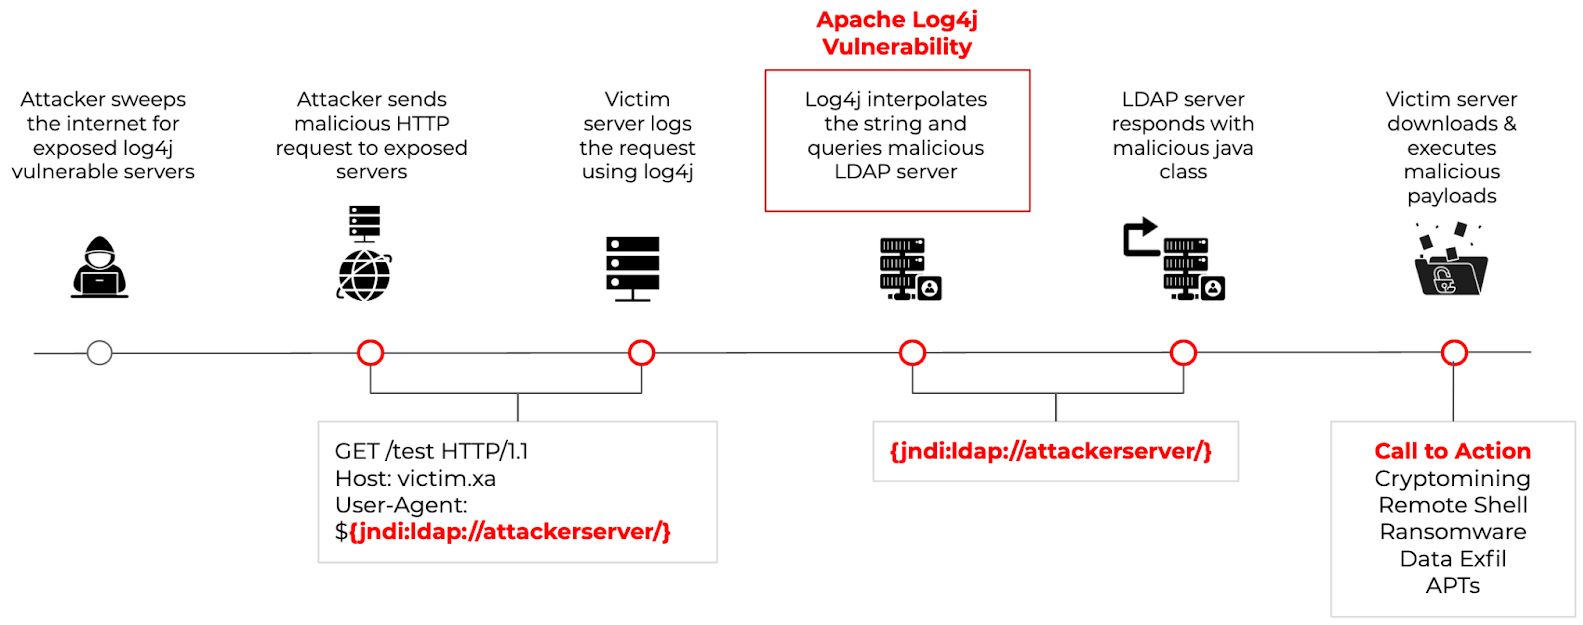
\includegraphics[width=1\linewidth]{img/log4shell-schema.png}
    \caption{Schematische voorstelling van een Log4shell aanval ~\autocite{Zscaler2021}.}
    \label{fig:log4shell-schema}
\end{figure}

{\bf Merk op:}
Door de overerfbaarheid van dependencies gaat de kwetsbaarheid ook overgeërfd worden en moet men dus de volledige hiërarchie gaan nakijken op kwetsbaarheden.


\subsection{Identificatie getroffen pakketten}

Onmiddellijk na de ontdekking van de CVE-2021-44228 verschijnen overal op het internet Proof of Concept aanvallen die misbruik maken van deze kwetsbaarheid. Hierdoor moeten cyberbeveiligingsbedrijven in een race tegen de tijd massale netwerkscans uitvoeren om kwetsbare applicaties en aanvallen op honeypots te ontdekken.

Om de Log4shell kwetsbaarheid te bestrijden moet men altijd eerst beginnen met een detectie zodat men weet of het systeem al gecompromitteerden is of niet. Het is van groot belang dat men alle bibliotheken hiervoor kent, zelfs alle onderliggende (dependencies), die de Log4j Java bibliotheek gebruiken. Hiervoor zijn online veel tools ~\autocite{Roth2022} te vinden en grote bedrijven en organisaties verspreiden hun eigen beveiligingsrapporten of ontwikkelen zelf bruikbare detectie- en patchingstools.

Enkele voorbeelden:
\begin{itemize}[leftmargin=*]
    \item Computer Emergency Response Team Coordination Center (CERT/CC) ~\autocite{CERTCC2022}
    \item Microsoft ~\autocite{MSRC2021, MDTIT2022}
    \item Sonatype ~\autocite{Mishra2021}
    \item Check Point ~\autocite{Checkpoint2021}
\end{itemize}

\subsection{Bestrijding Log4shell kwetsbaarheid}

Hoewel Apache de Log4j-kwetsbaarheid probeert op te lossen met de nieuwe patches, blijft het informatiebeveiligingsrisico bestaan voor organisaties die de voorkeur geven aan de bestaande Java-bibliotheek. Hiervoor moeten enkele chirurgische ingrepen gedaan worden om deze verder te kunnen gebruiken, zoals de bijvoorbeeld jndiLookups en bijhorende klassen verwijderen of via de properties de lookups deactiveren afhankelijk van de versies die er gebruikt worden.
In Figuur ~\ref{fig:log4jaanval} zien we een schematische voorstelling van manieren om een Log4shell aanval te bestrijden.

Bestrijding is onder andere mogelijk door:
\begin{itemize}[leftmargin=*]
    \item Upgrade de Log4j versie naar 2.17.1 of hoger;
    \item Verwijder de JndiLookup en de bijbehorende klassen;
    \item Schakel lookups uit via properties.
\end{itemize}

\begin{figure}[!ht]
    \centering
    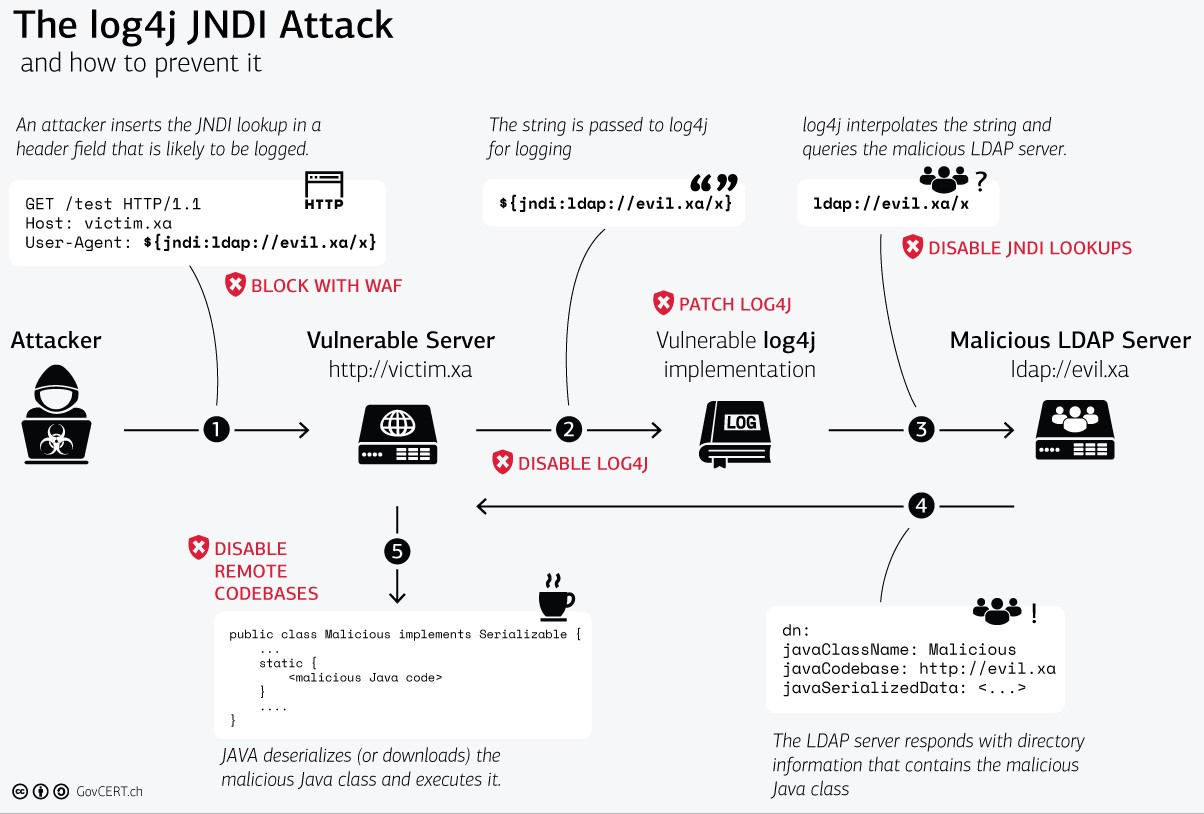
\includegraphics[width=1\linewidth]{img/log4jaanval.png}
    \caption{Schematische voorstelling van een Log4shell aanval met de manieren om de aanval te vermijden.}
    \label{fig:log4jaanval}
\end{figure}

\section{Proof-of-Concept}

\subsection{Intro}

Ter demonstratie van een Log4shell aanval is er een PoC ~\autocite{Akkurt2022} uitgewerkt die een beter beeld geeft over de werking van deze aanval en de detectie van de CVE-2021-44228 kwetsbaarheid.Er is een demo video te downloaden via \href{https://hogent-my.sharepoint.com/:v:/g/personal/thomas_thomas_y3313_student_hogent_be/EW-6cnKuqh1LmifrKeXAtLoB8SxmJZcj7Acj8Yl2-sFwqQ?e=1bDoFh}{\underline{deze link}}.De volledige labo omgeving kan opgezet worden via de ``poc'' subfolder van dit project door de stappen uit het beschrijvende README.md bestand te volgen.

\subsection{VirtualBox Omgeving}
Eerst wordt er op een geautomatiseerde manier een Debian 11 \autocite{boxomatic2022}, labo omgeving, opgezet via Vagrant die gebaseerd is op het Ansible Skeleton van \textcite{VanVrecken2020}. Alle nodige software voor deze Proof-of-Concept wordt automatisch geïnstalleerd en onmiddellijk klaargezet.

We kiezen een kwetsbare versie van de Java SE Development Kit, bijvoorbeeld versie 8u20 \autocite{Oracle2014} en plaatsen deze in de provisioning folder zoals ook uitgebreid in het README.md bestand en in de demovideo aangegeven is.

\subsection{Labo Omgeving}

De Log4jshell hack is gebaseerd op een eerder uitgebrachte PoC \autocite{Kozmer2022} en om deze uit te voeren zijn er 3 terminals nodig. In de eerste terminal openen we een Netcat listener, in de tweede terminal lanceren we de exploit (server aanvaller) en in de derde terminal starten we een Docker container met de kwetsbare webapplicatie.
In Figuur ~\ref{fig:log4shell-poc} wordt getoond hoe een geslaagde aanval eruit ziet.
\begin{figure}[!ht]
    \centering
    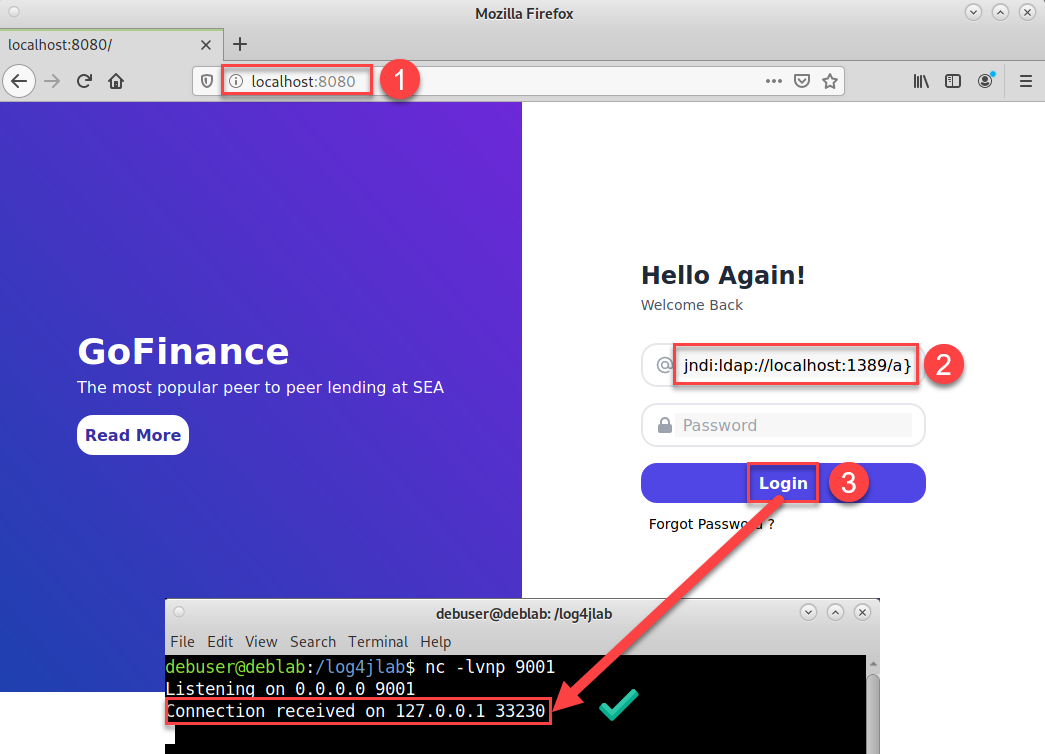
\includegraphics[width=1\linewidth]{img/log4shell-poc.png}
    \caption{Voorstelling van een geslaagde Log4j aanval uit de PoC ~\autocite{Akkurt2022}.}
    \label{fig:log4shell-poc}
\end{figure}

\subsection{Controle kwetsbaarheid}

Ter controle van de CVE-2021-44228 kwetsbaarheid gaan we een webversie van de Log4shell-tools \autocite{Bakker2022b} van de Githubrepo van \textcite{Bakker2022a} gebruiken.

\section{Methodologie}

Het onderzoek start met het opzetten van een labo omgeving die als PoC dient en later als demo wordt gebruikt ter bewustmaking aan de nood van een goede cybersecurity. Er wordt ook een honeypot implementatie uitgevoerd die gebaseerd is op de ~\textcite{Patzke2022}.
Aan de hand van de opgezette labo omgeving worden verschillende detectiemethodes vergeleken en wordt een analyse gemaakt van de inzetbaarheid bij soortgelijke aanvallen. Daarnaast wordt er een vergelijkend onderzoek gedaan van hoe de kwetsbaarheid kan verholpen worden met telkens de voor- en nadelen van de toegepaste methodes. Ook wordt er bekeken wat de impact van Log4shell was en is bij enkele bedrijven op financieel en technologisch vlak.

\section{Conclusie}

Het onderzoek zou een inzicht moeten geven over hoe gevaarlijk deze exploit is en soortgelijke exploits kunnen zijn. Hieruit zal een resultaat verkregen worden over de werking van dit soort exploits en hoe deze het beste te bestrijden zijn. Uiteindelijk zullen ook de voor-en nadelen worden bekeken en geanalyseerd van de investeringen in cybersecurity, zodat soortgelijke aanvallen in de bedrijfswereld tijdig gedetecteerd en gestopt kunnen worden. Verwachten wordt dat bedrijven nog steeds niet genoeg investeren in cybersecurity, waardoor er altijd een grotere kans bestaat dat ze door een cyberaanval worden getroffen.


\phantomsection
\printbibliography[heading=bibintoc]

\footnote{https://github.com/HoGentTIN/rm-2122-paper-rmakkurtthomas}
\end{document}
